\documentclass[12pt,a4paper]{report}
\usepackage[utf8]{inputenc}
\usepackage[francais]{babel}
\usepackage[T1]{fontenc}
\usepackage{amsmath}
\usepackage{amsfonts}
\usepackage{amssymb}
\usepackage{graphicx}
\usepackage{enumitem}
\usepackage{xcolor}
\usepackage{tikz}
\usetikzlibrary{arrows,automata}
\usepackage[left=2cm,right=2cm,top=2cm,bottom=2cm]{geometry}
\author{BA Alhassane}
\title{Rapport projet de deep learning \\ Autoencodeur\\Master 1 ANO \& IA \\Université Paris Scalay }
\begin{document}
\maketitle 
\tableofcontents
\section{Introduction}


Dans ce rapport du projet de deep learning. On va étudier l’entraînement des auto-encodeurs et un de ces cas particuliers des modèles génératifs notamment les auto encodeurs  variationnels. Cet entraînement se fera et se limitera essentiellement avec les outils du Module pytorch. 
On va essayer de parler d'abord une manière générale les caractéristiques   et les proriétés  les plus générales des autoencodeurs. Ensuite on va aborder les aspects techniques de l’entraînement. L'architecture des traitements dans les deux études sera la même. Elle sera composée nécessairement du modèle à entraîner, la fonction coût, l'optimiseur et autres paramètres et fonctionnalité d'optimisation provenant du module de pytorch.  

\section{Les auto-encodeurs }

\subsection{Définition \& carctéristiques}
Un auto encodeurs est un réseau de neurones entraîné pour tenter de reproduire en sortie les données d'entrées. Il comprend une couche cachée h qui décrit un code pour représenter l'entrée.Ce réseau est composé de deux parties :
\begin{itemize}
\item Une fonction d'encodage : l'encodeur  $h=f(x)$
\item Et une fonction de décodage : le décodeur qui produit une reconstruction $r=g(h)$ 

\end{itemize}


Le modèle est contraint de prioriser les caractéristiques des données qui doivent être reproduites. C'est  pour cette raison qu'il apprend les propriétés les plus pertinents  dans les données. \\
Les autoencodeurs modernes ont généralisé le principe d'encodage et de décodage , au delà du cadre déterministe , en considérant des transformations stochastiques $p_{encoder}(\textbf{h} |x)$ et $p_{encoder}( x|\textbf{h})$.\\
Ils sont capable d'apprendre sans aucune supervision. ie le jeu d'entrainement n'a pas d'étiquette ou label. Ils sont utilisés pour les préentariements non supervisés des réseaux neurones profonds.\\
Les auto-encodeurs peuvent être considérés comme un cas particulier de réseaux à propagation avant et peuvent être entraînés avec les même techniques typiquement une descente de gradient par mini-lots suivant des gradients calculés par rétropropagation.
\subsection{Les types de auto-encodeurs }
Il existe plusieurs types d'auto-encodeurs: 
\definecolor{blue}{RGB}{51,131,255}
\begin{itemize}[label=\textbullet, font=\LARGE \color{blue}]
\item les auto-encodeurs sous-complets:  \\
Ici $\textbf{h}$ est contraint à avoir des dimension plus petites que celle de $x$. L'apprentissage d'une représentation incomplètes force l'auto-encodeur à capturer les caractéristiques les plus discriminant des données d'apprentissage. Le processus d'apprentissage est décrit simplement comme minimisant $L(x,g(f (x) )$. Où $L$ est une fonction de perte pénalisant $g(f (x) $  si il est différent de $x$.

\item les auto-encodeurs régularisés :  \\
Parfois la dimension de $\textbf{h}$  est autorisée à être supérieure ou égale à celle de $x$,les auto-encodeurs régularisés utilisent une fonctions de perte qui encourage le modèle  à  acquérir des propriétés supplémentaires à sa capacité de reproduction des données d'entrées.
\item les auto-encodeurs parcimonieux: 
Est simplement un auto-encodeur dont le critère d’entraînement introduit une pénalité $	\Omega(\textbf{h})$ sur sur la couche de code en plus de l'erreur de reconstruction $L(x,g(f (x) )+ \Omega(\textbf{h})$. On peux voir le  $ 	\Omega(\textbf{h})$  comme un régulateur ajouté à un  résseau à propagation avant dont l'objectif est de reproduire les données d'entrées.

\item les auto-encodeurs débruiteurs :  \\
cet auto-encodeurs minimise $L(x,g(f (\bar {x}) )$ avec $\bar {x}$ une copie de $x$ ayant été corrompue. Le rôle du décodeur est d'annuler une corruption;\\


\end{itemize}

\subsection{Quelle taille de couche et de profondeur ? }
La taille des couche et des profondeur peut être variables et n'exige pas une condition nécessaire qu'elles soient supérieure ou égale à 1.Cependant l'utilisation d'encodeurs et de décodeurs profonds offre beaucoup d'avantages. Car  similaires aux réseaux à propagation avant.La profondeur peut réduire de façon exponentielle le de calcul de la représentation.

\subsection{Quel type de fonction de coût et d'unités cachées ? }
Les auto -encodeurs ne sont que des réseaux à propagation avant.Les même fonctions de pertes et les même type d'unités de sortie peuvent être   utilisés pour les réseaux traditionnels à propagation avant. On sait que la meilleur stratégie de définir les unités de sorties et la fonction de perte pour les réseaux  à propagation avant est de définir une distribution de sortie 
$p(\textbf{y}|\textbf{x})$ puis de minimiser la log probabilité $ - log($p(\textbf{y}|\textbf{x})$)$ avec $\textbf{y}$ le vecteur cible.Sauf que ici avec les auto-encodeurs $ \textbf{x}$ joue le rôle d'entrée et de cible.
\section{les concepts et techniques des auto-encodeurs abordés dans ce projet}
Les auto-encodeurs sont largement utilisées avec des différents concepts et techniques d'apprentissage avec des théorie différentes. ici dans ce projet on va largement les principes de l'apprentissage non-supervisés et semi-supervisés.Dans le procahain paragraphe on va essayer de d'expliquer le principe de représentation pour pouvoir comprendre comment les apprentissages non-supervisés  et semi-supervisés se font.
\subsection{Apprentissage de représentation : non supervisé et semi-supervisé}
On peut considérer les réseaux de neurones à propagation avant entraînés par apprentissages non supervisés comme une forme de représentation.La dernière couche du réseaux est plus souvent un classificateur softmax. Et le reste du réseau fourni à représenter un classificateur.L'apprentissage de représentation est particulièrement  intéressant parce qu'il offre une méthode pour effectuer un apprentissage non supervisé et semi-supervisé.
\subsection{L'entrainement des modèles probabilistes \& problème d'optimisation}
De nombreux modèles probabiliste sont difficiles à entraîner  car ils sont difficiles à inférer. les problèmes 'inférences en apprentissage profond découlent  généralement  de l’interaction entre les variable latentes. Le problèeme de l'inférence est de calculer $p(\textbf{h}|x)$  Il existe deux types de 
d'inférence. L'inférence approchée et l'inférence exacte. l'inférence exacte peut être considérer comme un problème d'optimisation. Il est très difficile de calculer $logp(v;\theta) $ s'il est coûeux de marginaliser $ h$. Au lieu de cela nous pouvons calculer une borne de $L(v,\theta,q) $ sur  $logp(v;\theta) $. Cet borne inférieure s'appelle le \textit{Evidence Lower Bound}.On va détailler son expression dans la suite.
\section{Les auto-encdeurs variatonnels AEV}
Ce sont des auto-encodeurs qui peuvent être entraînés par des méthodes fondées sur le gardiens. Ce sont des auto-encodeurs génératifs.ie ils sont capables de générer de nouvelles instances qui semble provenir du jeu d’entraînement. Les auto-encodeurs variationnels détermine comment entraîner des réseaux génératif différentiables lorsque la valeur de $z$ pour chaque $x$ n'est pas fixe. \\
Pour générer un échantillon à partir du modèle, AEV tire d'abord un échantillon $z$ de la distribution de code  $p_{model}(z)$.L'échantillon nourrit ensuite un réseau génératif différentiable $g(z)$. Enfin $x$ est échantillonné à partir d'une distribution $p_{model}(\textbf{x};g(z)=p_{model}(\textbf{x}|z)$. Pendant l’entraînement , cependant ,le réseau d’entraînement d'inférence ou encodeur $q(z|\textbf{x})$ est utilisé pour obtenir $z$ et  $p_{model}(\textbf{x}|z)$ est considérer comme le réseau de décodage. Leur principe clé est que il peuvent être entrainer en maximisant la borne inférieure variationnelle $l(q)$ qui inférieur ou égale à $\log (p_{model}(\textbf{x}))$.
\begin{equation}
\mathcal{L}(q)=\mathbb{E}_{z \sim  q} \log p_{model} (\textbf{x}[z)+ D_{KL}(q(\textbf{z}|x) || p_{model}(\textbf{z})) 
\end{equation}

\begin{equation}
\mathcal{L}(q) \leq \log  p_{model}(\textbf{x})
\end{equation}

Dans l’équation (1) , le premier terme correspond à la reconstruction de la $log-vraissemblance$ que l'on trouve dans d'autres auto-encodeurs. Le deuxième terme essaie de faire en sorte que la distribution approchée $q(z|\textbf{x})$ et le modèle précédent $p_{model}(z)$ converge vers l'un vers l'autre. Un VEV permet d'entraîner un ecodeur paramétrique  (réseau d'inférence ou modèle de reconnaissance) qui produit les paramètre de  $q$. Tant que $z$ est une variable continue on peut effectuer une retro propagation   à partir de $z$ issus de 
$q(z|\textbf{x}) =   q(z;f(\textbf{x}; \Theta )$  pour obtenir un gradient par rapport à $ \Theta$. L'apprentissage consiste uniquement à maximiser  $\mathcal{L}$ 
par rapport aux paramètre de l'encodeur et du décodeur.

\section{Retropropagation à travers des opérations aléatoires}
Les réseaux de neurones traditionnels mettent en œuvre une transformation déterministe de certaine  variable d'entrées $\textbf{x}$.
Les modèles génératifs ont tendance à faire des transformations stochastiques. Une façon de le faire est d’augmenter le  réseau de neurone avec des entrées supplémentaires $\textbf{z}$ qui sont échantillonnés à partir d'une distribution de probabilité simple telle qu'une distribution uniforme ou gaussienne. Le réseau de neurone peux alors continuer à effectuer des calculs  déterministes en interne, mais la fonction $f(\textbf{x},z)$ apparaîtra stochastique à un observateur qui n'a pas accé  à $z$.Si $f$ est continu et différentiable nous pouvons calculer le gradient nécessaire par rapport à l’entraînement en utilisant la rétro propagation comme d'habitude.

\subsection{Exemple avec la distribution gaussienne}
A titre d'exemple ,considérons l'opération  consistant à tirer des échantillons $y$ d'une distribution gaussienne une moyenne $\mu$   et variance $\sigma$.On a 
\begin{equation}
y \sim  \mathcal{N}(\mu,\sigma^{2})
\end{equation}
Parce qu'un échantillon individuel $y$ n'est pas produit pas une fonction mais par un processus d’échantillonnage dont la sortie change à chaque fois que nous l'effectuons. Il peux paraître contre intuitif de calculé les dérivées de $y$ par rapport aux paramètres de sa distribution. cependant , nous pouvons réécrire le processus d’échantillonnage comme la transformation d'une valeur aléatoire sous-jacente $\textbf{z} \sim  \mathcal{N}(z,\mu=0,\sigma^{2}=1)$ permettant d'obtenir un échantillonnage à partir de la distribution souhaitée.\\
\begin{equation}
\textbf{y}=\mu+\sigma z
\end{equation}
Nous sommes maintenant à mesure de d'effectuer une rétropropagation à travers l'opération déchantillonnage en la considérant comme une  opération déterministe avec une entrée suplémentaire $z$ déterministe. L'entrée supplémentaire est une variable aléatoire dont la distribution n'est fonction d'aucune variable aléatoire dont nous voulons calculer le dérivée. 

\subsection{Fonctions loss }

La fonction de coût comprend deux parties , la première est la perte de reconstruction habituelle qui poussent l' auto-encodeur à reproduire ses entrées.La seconde est la perte l'attente qui pousse l'auto-encodeur à produire des codages semblant avoir été échantillonnés à partir d'une simple distribution normale. 

\begin{equation}
L=MSE(y',y)=+KL(q(z|x),p(z))
\end{equation}

avec $MSE(y',y)=\frac{1}{N}\sum_{i=1}^{k}(y'-y))$ et  $KL(q(z|x),p(z))=\frac{1}{2}\sum \mu_{i}^2 +\sigma_{i}^2 -\frac{1}{2} -\log(\sigma_{i}^2)$

\section{ Le choix des  techniques de l'apprentissage et des types de couches utilisées }
On rappelle que chaque un auto-encodeur est constitué d'un  encodeur et d'un décodeur. On rappelle aussi que chacun d'eux à une structure de multiple couches. Et sont des réseaux à propagation avant.

On sait aussi  que les perceptions sont  de basique type de des architectures des réseaux de neurones artificiels. Leur apprentissage est basé sur la recherche du paramètre \textbf{w} qui rapproche les prédictions aux cibles.
Les réseaux de neurone à multiple couche généralisent le principe des perception sur des architectures plus complexes à plusieurs noeuds d'entrées. 
Les noeuds sont arrangés pour désigner un couche. L'architecture d'un réseau de neurones n'est rien d'autre qu'une superposition des  ces couches. 

Toutes les hypothèses et techniques d'apprentissage utilisées jusque là pour l'apprentissage supervisé vont s'appliquer sur les auto-encodeur plus particulièrement sur chaque partie de l'auto-encodeur. 

\subsection{Le choix du nombre de couche  et des fonction  d'activation dans ce projet } 


\definecolor{blue}{RGB}{51,131,255}
\begin{itemize}[label=\textbullet, font=\LARGE \color{blue}]
\item  \textbf{Le nombre de cuche  } : \\
J'ai choisi plusieurs couches pour les  encodeurs et les décodeurs. Car plus il y'a de couche plus les prédictions sont meilleurs. 

\item  \textbf{Les  fonction d'activation de sorties : sigmoid} \\
Mais le choix des fonctions d'activations et les fonctions de coûts sont un vrai problème du deep learning car un mauvais choix peut provoquer facilement des saturations sur la sortie. 
Ici dans ce projet la fonction d'activation des couche de sortie est donnée parla fonction  $sigmoid$. C'est bien adapté  pour les valeurs qui s’étende entre 0 et 1.
\item \textbf{loss fonction }\\
On a choisi le MSE car inspiré des modèles de perceptrons et des techniques de  l'apprentissages basé sur backpropagation. En suite on ajoute un terme du $ D_{KL} $ sur les paramètres distributions.
\item   \textbf{Les  fonction d'activation des couches cachées  : RelU}\\
Pour les couches cachés j'ai utilisé la fonction $ReLU$. Il est très utile pour éviter les problème  de  calculs de gradient avec la technique de backpropagation qui s'appelle le  \textit{"the vanishing gradient problems"}  

 
\end{itemize}*

\newpage

\section{Apprentissage }
\definecolor{blue}{RGB}{51,131,255}
\begin{itemize}[label=\textbullet, font=\LARGE \color{blue}]
\item \textbf{ Pour la partie 1 }
\begin{itemize}
\item On on a choisit  une taille  batch =64  pour le traitement avec toutes les 784 features. Avec 10 EPOCH d'itérations.
\item Pour le leraning rate on a choisi lr=1e-3
\item les résultats du loss avec EPOCH = 10 étérations avec BATCH=64. :

\begin{figure}[!h]
   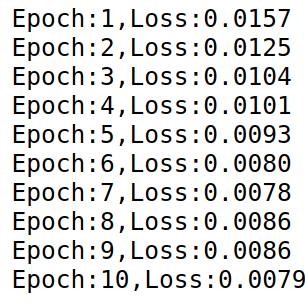
\includegraphics[scale=0.6]{training.png}
\end{figure}
%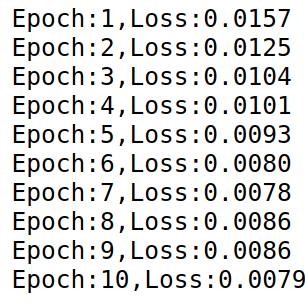
\includegraphics{training.png}

\end{itemize}


\item \textbf{ Pour la partie 2 }\\
Avec les même paramètre d'entrés que avant on obtient 

\begin{figure}[!h]
   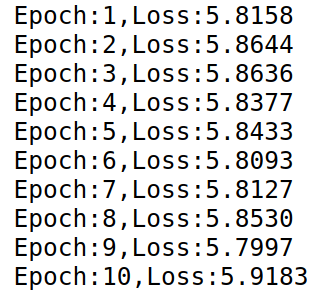
\includegraphics[scale=0.6]{training1.png}
\end{figure}
%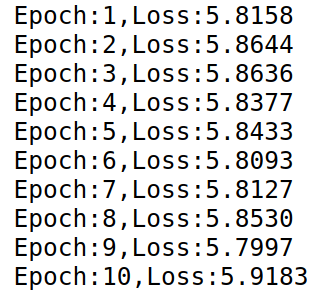
\includegraphics{training1.png}


\item  \textbf{Commentire} : \\
Le première partie est un problème d'auto-encodeur classique. Les résultats ne sont pas  mal peour uniquemment 10 itérations. La fonction couts et les paramèters d'optimisations sont donnés par les modules de pytorchs. A partir de 10 itération on obtient des images claires. 

Pour la deuxièpme partie :
 C'est le contraire. Pour les premières   10 itération toutes les images sont floues. C'est du à plusieurs facture comme la terme de $KL$ sur la paramètre de distribution de distribution gaussienne qui s'ajoute sur la fonction coût globle.
 Les les du loss global sont très grandes. Mais avec des itération plus grand par exemple 17 à 20 itérations  on peut obtenir des images un peux flous. Mais les temps de calculs sont très longs. 
 

\end{itemize}



\section{Conclusion }

Cette partie des auto-encodeur reprend toutes étapes et techniques  d'apprentissages vu précédemment de l'apprentissage des perceptron jusqu'au  résaux de neurones forward pass et backpropagation  . Elle  utilise ces concepts avec un approfondissement et généralisation sur le plan théorique et technique du deep learing.   
Cette étape de développemnet d'architecture nous a permis de comprendre la vraie modélisation des couches cachées et des variables latentes surtout  avec pytotorch.
Ce projet et ce cours  nous a permis de comprendre le principe et les applications du deep learning d'une manière large. Il donne  les bases nécessaire pour continuer  et aborder indépendamment sles autres études études du deep learning.\\


\textbf{REFERENCES :}
Toutes les parties de la théorie écrites ici  sont prises dans les ouvrages suivantes:  

\definecolor{blue}{RGB}{51,131,255}
\begin{itemize}[label=\textbullet, font=\LARGE \color{blue}]
\item Titre :L'apprentissages profond.\\
 Auteurs :Ian Goodfellow,Yoshua Bengio,Aaron Courville
 \item Titre :Deep Learning avec Kéras et TensorFlow. Mis en oeuvre et cas concrets\\
 Auteur Aurélien Géron
 
 \item Titre :Introduction to data mining. second edition
 Auteurs:
 Pang-Ning Tan,Michael Steinbach,Anuj karpatne,Vipin Kumar
 
 
 
 
\end{itemize}

\end{document}


